
\chapter{Introducción}

La piel es considerada el órgano mas grande del cuerpo humano,  y está compuesta por tres capas: \emph{\gls{epidermis}}, \emph{\gls{dermis}} e \emph{\gls{hipodermis}} (Véase Fig \ref{fig:skin1_jpg}). La principal función de la piel es proteger al cuerpo de las hostilidades del medio ambiente como la radiación solar y los factores externos como las bacterias, sin embargo también cumple otras funciones importantes aparte de proteger los órganos y los tejidos internos, tales otras funciones son regular nuestra temperatura corporal, registrar sensaciones de presión, frío, calor y es una interfaz para poder sentir e interactuar con lo que tenemos a nuestro alrededor.


\begin{figure}[h!]
    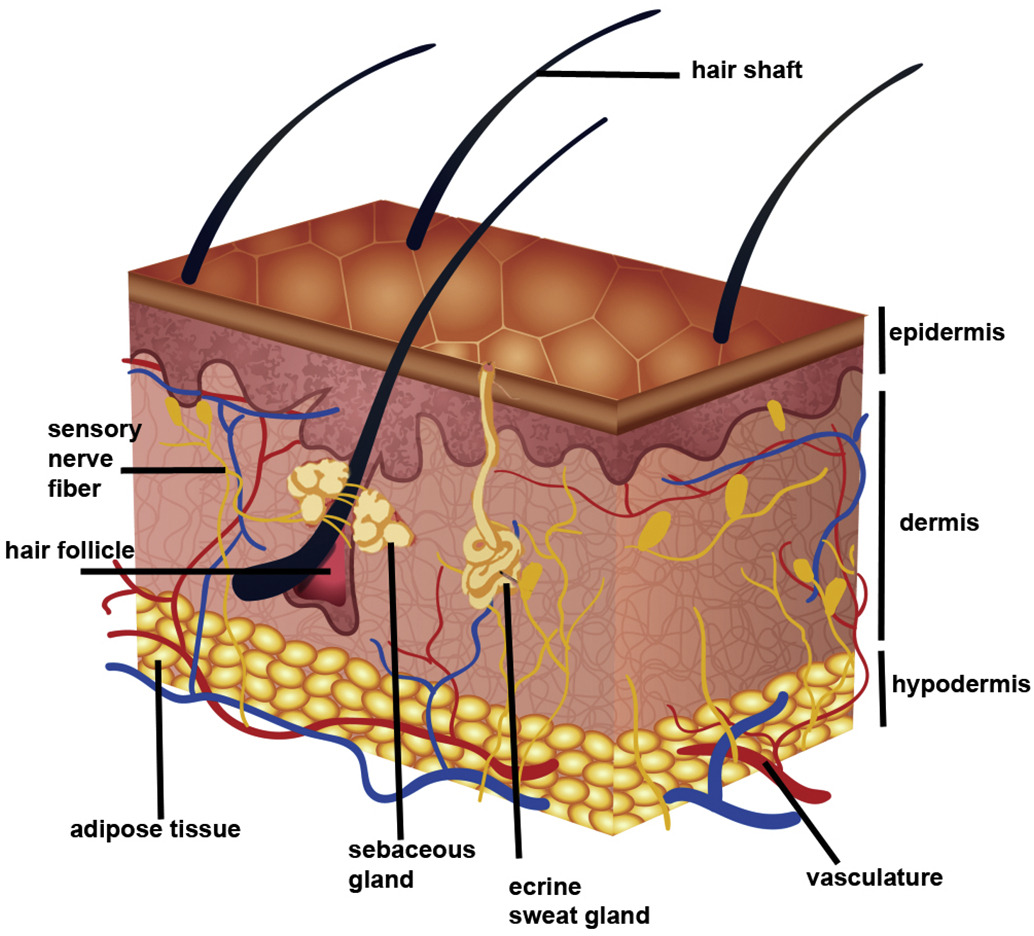
\includegraphics[width=80mm, scale = 0.5]{Figuras/skin_structure1.jpg}
    \centering
    \caption{Ilustración de las capas de la piel y sus apéndices \citep{skin_1}.}
    \label{fig:skin1_jpg}
\end{figure}

Sin embargo, debido a la exposición continua a las radiaciones de la luz, es común desarrollar enfermedades en la piel que afectan la forma en que las células de ésta se reproducen, causando graves daños a nuestra salud que en muchas ocasiones puede llegar a ser letal. Estas anomalías en la piel se denominan como \emph{cáncer de piel}, principalmente en las siguientes tres categorías: cáncer de células basales, cáncer de células escamosas y melanomas \citep{cancer_org}.

\begin{figure}[h!]
    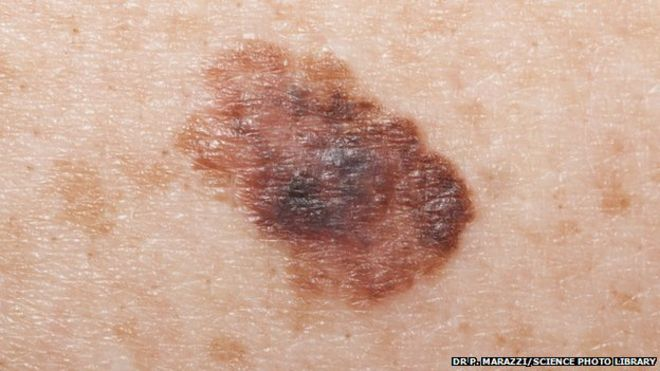
\includegraphics[width=80mm, scale = 0.8]{Figuras/skin_cancer_bbc.jpg}
    \centering
    \caption{Ejemplo de melanoma \citep{cancer_img_1}}
    \label{fig:can_jpg}
\end{figure}
 Su detección temprana es imprescindible para reducir las probabilidades de fallecimiento. Por lo tanto es necesario seguir desarrollando tecnologías que faciliten la detección de este tipo de padecimientos de forma rápida y sencilla que vaya enfocada en aumentar la accesibilidad a dichos diagnósticos y de esta forma reducir la tasa de mortalidad por este padecimiento.

En los últimos años se han logrado muchos avances en cuanto al desarrollo de software inteligente que han permitido un mayor acceso a diferentes servicios, una de estas tecnologías sería la \emph{\gls{rn}}, se trata de una tecnología que tiene la capacidad de aprender mediante el úso de datos históricos y funciones de optimización para crear un modelo matemático capaz de predecir, clasificar o recrear datos futuros o desconocidos. Algunos de los sectores que han comenzado a adoptar esta tecnología son: el sector automotriz (piloto automático), el sector de manufactura (optimización de procesos), el sector de entretenimiento (recomendaciones personalizadas), el sector médico (diagnóstico de imágenes). 


\section{Hipótesis}
Es posible clasificar los píxeles en distintas categorías dentro de una imagen gracias a las avances actuales de inteligencia artificial y la técnica de segmentación. Mediante la técnica de \emph{\gls{seg}} es posible crear un reconocedor visual que no solo detecte la presencia y ubicación del elemento a reconocer, sino que, también obtenga otros datos descriptivos del elemento como el tamaño, forma y región que abarca dentro de la imagen. De esta forma se puede obtener un diagnóstico automatizado certero.
\section{Objetivos}
Primero en \emph{Objetivo General} se habla de manera conceptual la problemática a resolver tales como cuales son las situaciones en las que podemos optimizar la resolución de un problema mediante el uso de la red neuronal, posteriormente en los \emph{Objetivos Específicos} se describe de forma puntual los pasos a realizar en el presente trabajo de tésis para llegar al resultado deseado.
\subsection{Objetivo General}
El \emph{objetivo general} de este trabajo de tésis es la localización de anomalías en la superficie piel que correspondan a alguno de los tipos de cáncer de esta región (basalioma, carcinoma, melanoma) mediante imágenes, con el uso de la red neuronal de \emph{\gls{seg}} basada en el modelo propuesto por \citet{wu2019fastfcn}, con la finalidad de desarrollar un modelo de red neuronal profunda capaz de segmentar de forma semántica las imágenes y sus correspondientes categorías.
\subsection{Objetivo Específico}
El \emph{objetivo específico} del experimento es el implementar una red neuronal cuya función sea la de recibir una imagen de entrada, extraer el mapa de características de dicha, y posteriormente reconstruya la imagen remarcando la región donde se encuentra el objeto a localizar. Para esto será necesario desarrollar un modelo y determinar las transformaciones necesarias por las que tendrán que pasar todas las imágenes con el fin de obtener el resultado deseado y también la mejor precisión posible.

\begin{figure}[h!]
    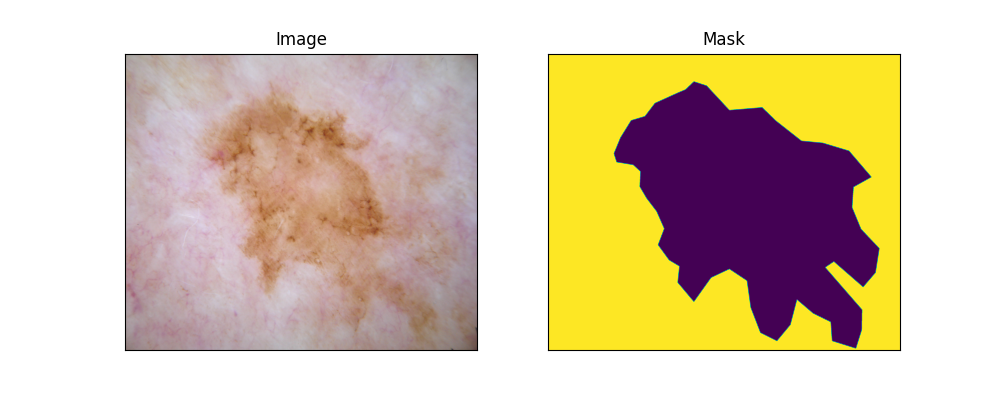
\includegraphics[width=150mm]{Figuras/plot_masks.png}
    \centering
    \caption{Ejemplo de la imagen de entrada (izquierda) y resultado esperado (derecha).}
    \label{fig:desired}
\end{figure}

\section{Estructura de la Tesis}

A continuación se dá una breve descripción sobre los capítulos que se verán a continuación en este documento.

En el capítulo 2 se habla sobre los conceptos relacionados al experimento, primero se hablará de los conceptos generales que se usarán a lo largo de este capítulo y posteriormente se hablará sobre los componentes de la red neuronal, los tipos de redes mas comúnes. 

En el capítulo 3 se habla sobre el estado del arte en cuanto a las redes neuronales, cuales son los avances en los últimos años y que ventajas tenemos ahora comparado al avance que se tenía cuando experimentos fueron realizados.

En el capitulo 4 se describe de forma estadística los datos que serán utilizados para realizar el experimento, tomando en cuenta la distribución de los pixeles en distintas regiones de la imagen, entre otros parámetros. 

En el capítulo 5 se detalla el proceso de implementación, primero se describirán las características del hardware, se describe la arquitectura del modelo y las transformaciones por las que pasará la imagen y luego se hará una comparativa con distintos modelos de redes neuronales para comparar tiempo de entrenamiento, precisión y resultado.

Finalmente, en el capítulo 6 se exponen los resultados obtenidos de la implementación del producto científico en el capítulo anterior, así como un análisis y conclusión final sobre los valores obtenidos en precision y tiempo de entrenamiento. 

\chapter{Antecedentes}
En este capítulo se introducen de forma teórica los conceptos relacionados a los tipos de cáncer y las redes neuronales, primero se define que es el \emph{cáncer de piel}, cuales son los factores que influyen en el desarollo de este padecimiento, los tipos de cáncer y las diferencias entre estos. Después algunos conceptos relacionados con las redes neuronales necesarios para un entendimiento sólido del \emph{aprendizaje profundo}, tales como los elementos clave que conforman a la red neuronal, la manera en la que esta evalúa su precisión, y el algoritmo de optimización.

\section{Cáncer de Piel}
El \emph{cáncer de piel} es una enfermedad que suele relacionarse con la aparación de lunares o manchas que no se encontraban previamente, se pueden manifestar como manchas oscuras o rojizas, bultos y/o escamas en la superficie de la piel. Esta enfermedad se desarrolla principalmente en partes de la piel expuestas al sol, sin embargo también se puede desarrollar en partes que no suelen exponerse. Algunos factores como la exposición a los rayos ultravioletas (UV), el uso de sustancias como el tabaco o el envejecimiento de la piel pueden ser factores correlacionados con el \emph{c{ancer de piel}}, dichos factores se dividen en dos grupos: 

\begin{itemize}
    \item Factores intrínsecos
    \item Factores extrínsecos
\end{itemize}

Los factores \emph{intrínsecos} son aquellos que suceden de forma interna en la piel, un ejemplo de esto es el envejecimiento cronológico, el cual es un proceso natural que consiste en degradación del colágeno, la elastina y el adelgazamiento de la epidermis debido al envejecimiento celular al paso de los años y de el efecto de algunas hormonas.

Los factores \emph{extrínsecos} son aquellos que suceden de forma agena al organismo, como es el caso del \emph{foto-envejecimiento} el cual sucede cuando nos encontramos expuestos a los rayos ultravioletas (UV). Este factor de envejecimiento genera lesiones en las cadenas de ácido desoxirribonucleico (ADN) debido a la oxidación y afecta la regeneración de celulas, al sistema inmune y a la forma en la que se regula la pigmentación \citep{skin_aging}.

\subsection{Tipos de Cáncer de Piel}
Existe una gran variedad de tipos de \emph{cáncer de piel}. Son cuatro tipos los que destacan por su incidencia.

\begin{itemize}
    \item melanoma
    \item cáncer de piel no melanoma
    \item carcinóma de celulas basales
    \item carcinóma epidermoide de piel
\end{itemize}

\section{Redes Neuronales}

Hasta hace algunos años el desarollo de aplicaciones de software solían desarrollarse mediante un proceso específico, generalmente se suele reunir a un grupo de desarrolladores para estudiar un problema y determinar una solución mediante el úso de las distintas plataformas de código disponibles y así ofrecer una solución a dicho problema, sin embargo con los avances actuales en el área de inteligencia artificial es posible resolver los mismos problemas de una forma distinta mediante el uso de datos históricos. 

\subsection{Datos de Imágenes}
Las \emph{imágenes} se pueden definir como una matriz de $\mathbf{m}$ x $\mathbf{n}$ pixeles (en el caso de las imagenes en blanco y negro).

\subsection{Modelos}
Un \emph{modelo} se puede definir como el bloque intermedio entre nuestros datos de entrada (input) y los datos de salida (output), en el modelo podemos encontrarnos con los siguientes elementos:

\begin{itemize}
    \item Nodos de entrada (Input nodes)
    \item Nodos intermedios (Hidden nodes)
    \item Nodos de salida (Output nodes)
    \item Capas (Layers)
    \item Pesos (Weights)
    \item Funciones de activación (Activation)
    \item Bías (Bias)
\end{itemize}

Los cuales se explican a continuación:

\subsection{Evaluación}
Para poder realizar el proceso de \emph{aprendizaje} de nuestro modelo, este debe tener la capacidad de evaluar la precisión actual. Para esto existen distintas funciones que nos permiten evaluar la precisión dependiendo del valor actual y el valor al cuál nos queremos acercar.

\subsection{Optimización}
Ya que tenemos calculada la diferencia entre el valor que estabamos prediciendo y el valor real (ground truth), es necesario hacer ajustes al modelo para poder acercarnos al valor real. 

\chapter{Estado del Arte}
A continuación se hará un estudio de los trabajos relacionados con el problema señalado en este trabajo de tesis y también con el método propuesto para solucionarlo.

\section{Trabajos Similares}

\section{Área de Oportunidad}

\chapter{Descripción de los Datos}

\chapter{Implementación de la Solución}

\chapter{Resultados}

